\chapter{UJI COBA DAN IMPLEMENTASI}

\section{Lingkungan Uji Coba}

Uji coba dilakukan pada perangkat dengan spesifikasi berikut.
\begin{enumerate}
	\item Perangkat Keras
	\begin{enumerate}
		\item Processor Intel® Core™ i5-7400 CPU @ 3.00GHz (4 CPUs), ~3.0GHz
		\item Random Access Memory 8192MB
	\end{enumerate}
	\item Perangkat Lunak
	\begin{enumerate}
		\item Sistem Operasi Windows 10 Pro 64-bit
	\end{enumerate}
\end{enumerate}
\section{Skenario Uji Coba}

Subbab ini akan menjelaskan hasil pengujian program penyelesaian permasalahan. Pengujian dilakukan untuk dua metode: metode \textit{Baby-step Giant-step} dan metode \textit{Pollard Rho}. Ada dua metode pengujian yang akan digunakan:

\begin{enumerate}
\item Pengujian lokal. Pengujian ini menggunakan mesin yang digunakan dalam pengembangan untuk mengukur kebenaran dan informasi lain mengenai program.
\item Pengujian luar. Pengujian ini menggunakan Online Judge untuk mengukur kebenaran dan informasi lain mengenai program.
\end{enumerate}

Pada pengujian lokal, dibutuhkan beberapa data sebagai masukan. Untuk itu program pembuat data uji akan digunakan dimana program tersebut diatur supaya menghasilkan kelompok data masukan dengan karakteristik berikut.

\begin{enumerate}
\item Kelompok data masukan dengan nilai N tetap. Nilai masukan lain menyesuaikan.
\item Kelompok data masukan dengan nilai L tetap. Nilai masukan lain menyesuaikan.
\end{enumerate}

Untuk lebih merepresentasikan data masukan, nilai $ q $ dan $ p $ pada tiap data masukan diatur supaya berada pada rentang $ 2^{N-1} \leq q < 2^N $ dan $ 2^{L-1} \leq p < 2^L $. Data masukan didesain agar merentang sebanyak mungkin kasus uji. Pada data masukan dimana $ N $ bernilai tetap, nilai $ L $ merentang pada nilai $ N+3 \leq L \leq 60 $\footnote{Pada praktiknya, pengujian dilakukan hanya sampai $ N = 53 $ karena keterbatasan sumber daya}. Sedangkan pada data masukan dimana $ L $ bernilai tetap, nilai $ N $ merentang pada nilai $ 10 \leq N < L $.  Setiap pasangan parameter (\textit{N, L}), dibuatkan maksimal 10 kasus uji yang berbeda-beda.

\section{Uji Coba Kebenaran}

Kebenaran setiap metode diujikan dengan mengirim kode sumber terkait ke Timus Online Judge. Berikut bukti hasil pengujian.

\begin{enumerate}
\item Kode sumber dengan metode Pollard Rho. (Gambar \ref{fig:verdict_pollard})
\begin{figure}[h!]
	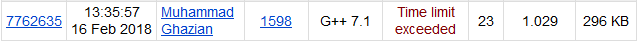
\includegraphics[scale=0.6]{bab5/img/pollard-verdict}
	\caption{Umpan Balik Online Judge Metode Pollard Rho}
	\label{fig:verdict_pollard}
\end{figure}
\item Kode sumber dengan metode Baby-step Giant-step. (Gambar \ref{fig:verdict_bsgs})
\begin{figure}[h!]
	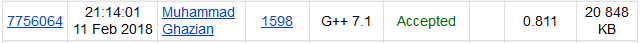
\includegraphics[scale=0.6]{bab5/img/bsgs-verdict}
	\caption{Umpan Balik Online Judge Metode \textit{Baby-Step Giant-Step}}
	\label{fig:verdict_bsgs}
\end{figure}
\end{enumerate}

Umpan balik yang didapat kode sumber dengan metode \textit{Pollard Rho} adalah \textit{Time Limit Exceeded}. Karena pengujian kebenaran metode tersebut tidak dapat dilakukan dengan pengujian luar, pengujian lokal akan digunakan. Hasil pengujian metode tersebut untuk setiap kelompok masukan dapat dilihat pada tabel \ref{tab:test_result_fixed_l} dan \ref{tab:test_result_fixed_n}.

\begin{table}[h!]
\caption{Uji Kebenaran Metode Pollard Rho Dengan Data Masukan L Tetap}
\label{tab:test_result_fixed_l}
\begin{tabularx} {\linewidth}{ |l l X X|l l X X| }
\hline
N	&L	&Jumlah Kasus Uji	&Jumlah Benar	&N	&L	&Jumlah Kasus Uji	&Jumlah Benar \\
\hline
10&	60&	10&					10&				32&	60&	10&	10 \\ 
11&	60&	10&					10&				33&	60&	10&	10 \\ 
12&	60&	10&					10&				34&	60&	10&	10 \\ 
13&	60&	10&					10&				35&	60&	10&	10 \\ 
14&	60&	10&					10&				36&	60&	10&	10 \\ 
15&	60&	10&					10&				37&	60&	10&	10 \\ 
16&	60&	10&					10&				38&	60&	10&	10 \\ 
17&	60&	10&					10&				39&	60&	10&	10 \\ 
18&	60&	10&					10&				40&	60&	10&	10 \\ 
19&	60&	10&					10&				41&	60&	10&	10 \\ 
20&	60&	10&					10&				42&	60&	10&	10 \\ 
21&	60&	10&					10&				43&	60&	10&	10 \\ 
22&	60&	10&					10&				44&	60&	10&	10 \\ 
23&	60&	10&					10&				45&	60&	10&	10 \\ 
24&	60&	10&					10&				46&	60&	10&	10 \\ 
25&	60&	10&					10&				47&	60&	10&	10 \\ 
26&	60&	10&					10&				48&	60&	10&	10 \\ 
27&	60&	10&					10&				49&	60&	10&	10 \\ 
28&	60&	10&					10&				50&	60&	10&	10 \\ 
29&	60&	10&					10&				51&	60&	10&	10 \\ 
30&	60&	10&					10&				52&	60&	10&	10 \\ 
31&	60&	10&					10&				53&	60&	10&	10 \\
\hline
\end{tabularx}
\end{table}
\pagebreak

\begin{table}[h!]
\caption{Uji Kebenaran Pollard Rho Dengan Data Masukan N Tetap}
\label{tab:test_result_fixed_n}
\begin{tabularx} {\linewidth}{ |l l X X|l l X X| }
\hline
N	&L	&Jumlah Kasus Uji	&Jumlah Benar	&N	&L	&Jumlah Kasus Uji	&Jumlah Benar \\
\hline
10	&13	&7					&7				&10	&37	&10					&10 \\
10	&14	&8					&8				&10	&38	&10					&10 \\
10	&15	&10					&10				&10	&39	&10					&10 \\
10	&16	&10					&10				&10	&40	&10					&10 \\
10	&17	&10					&10				&10	&41	&10					&10 \\
10	&18	&10					&10				&10	&42	&10					&10 \\
10	&19	&10					&10				&10	&43	&10					&10 \\
10	&20	&10					&10				&10	&44	&10					&10 \\
10	&21	&10					&10				&10	&45	&10					&10 \\
10	&22	&10					&10				&10	&46	&10					&10 \\
10	&23	&10					&10				&10	&47	&10					&10 \\
10	&24	&10					&10				&10	&48	&10					&10 \\
10	&25	&10					&10				&10	&49	&10					&10 \\
10	&26	&10					&10				&10	&50	&10					&10 \\
10	&27	&10					&10				&10	&51	&10					&10 \\
10	&28	&10					&10				&10	&52	&10					&10 \\
10	&29	&10					&10				&10	&53	&10					&10 \\
10	&30	&10					&10				&10	&54	&10					&10 \\
10	&31	&10					&10				&10	&55	&10					&10 \\
10	&32	&10					&10				&10	&56	&10					&10 \\
10	&33	&10					&10				&10	&57	&10					&10 \\
10	&34	&10					&10				&10	&58	&10					&10 \\
10	&35	&10					&10				&10	&59	&10					&10 \\
10	&36	&10					&10				&10	&60	&10					&10 \\
\hline
\end{tabularx}
\end{table}
\pagebreak

Perhatikan bahwa di tabel \ref{tab:test_result_fixed_l} dan \ref{tab:test_result_fixed_n} nilai jumlah benar setiap kelompok masukan (yaitu pasangan N dan L) selalu sama dengan jumlah kasus uji yang digunakan. Maka dari itu, disimpulkan bahwa metode \textit{Pollard Rho} yang digunakan memberikan hasil yang benar. Detail terkait pengujian ini dapat dilihat pada lampiran A dan lampiran B.

\section{Uji Coba Kinerja}

Subbab ini akan menjabarkan kinerja setiap metode dengan lebih mendalam. Uji coba kinerja dilakukan melalui pengujian lokal. Menggunakan kasus uji yang sama dengan kasus uji pada subbab \ref{sec:Uji Coba Kebenaran}, akan dilakukan pengukuran waktu yang dibutuhkan untuk menyelesaikan permasalahan untuk setiap metode.

\subsection{Pengujian Menggunakan Parameter Masukan dengan N Tetap}

Pengujian menggunakan parameter masukan dengan $ N $ tetap dilakukan dengan langkah berikut.
\begin{enumerate}
	\item Rekam waktu tepat sebelum komputasi penyelesaian masalah dilakukan.
	\item Lakukan komputasi terkait penyelesaian masalah untuk sebuah masukan yang sama sebanyak 10000 kali secara berturut-turut
	\item Rekam waktu tepat setelah komputasi penyelesaian masalah dilakukan.
	\item Kurangi waktu saat selesai komputasi dengan waktu saat sebelum komputasi.
	\item Ulangi untuk seluruh kasus uji.
\end{enumerate}

Prosedur ini penting untuk dilakukan untuk memperjelas fluktuasi waktu yang dibutuhkan dalam menyelesaikan permasalahan. Keluaran prosedur ini yaitu lamanya waktu yang dibutuhkan untuk menyelesaikan permasalahan untuk 10000 kali percobaan. Perlu diperhatikan bahwa penggunaan metode \textit{Pollard Rho} menggunakan fungsi \textit{pseudorandom}, sehingga satu kali percobaan menggunakan metode \textit{Pollard Rho} sangat mungkin menghasilkan waktu yang berbeda.

\begin{figure}[h!]
	\Centering
	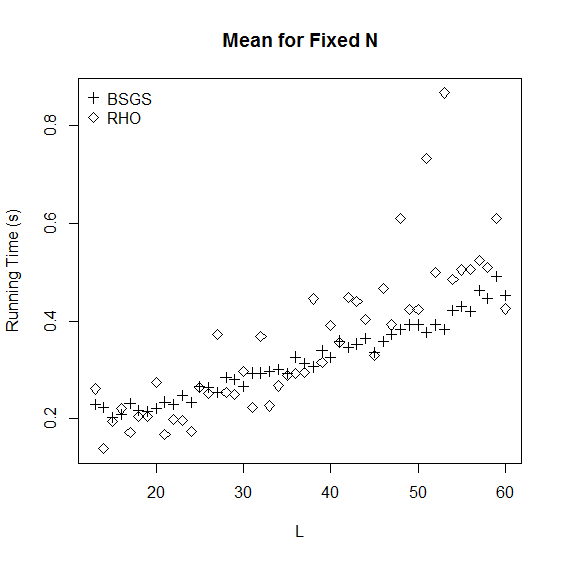
\includegraphics[angle=0, scale=0.55]{bab5/img/mean-fixed-n}
	\caption{Grafik Rata-rata Kinerja Dua Metode Untuk Kelompok Masukan N Tetap}
	\label{fig:mean_fixed_n}
\end{figure}

Grafik \ref{fig:mean_fixed_n} menampilkan rata-rata kinerja masing-masing metode apabila parameter masukan N bernilai tetap. Pada grafik tersebut dapat dilihat bahwa rata-rata \textit{running time} yang dimiliki kedua metode tidak berbeda jauh. Pada sekitar $ L \geq 40 $, rata-rata \textit{running time} metode \textit{Pollard Rho} cenderung lebih besar daripada \textit{Baby-step Giant-step}. Selain itu, \textit{running time} metode \textit{Pollard Rho} pada $ L \geq 40 $ cenderung berpencar, kontras dengan \textit{running time} \textit{Baby-step Giant-step} yang cenderung stabil.

Pertanyaan berikutnya adalah seberapa dekat \textit{running time} yang akan didapat antara rata-rata kinerja metode dengan \textit{actual running time} untuk kelompok masukan tertentu. Pertanyaan ini dapat dijawab dengan grafik 
\ref{fig:stddev_fixed_n}.

\begin{figure}[h!]
	\Centering
	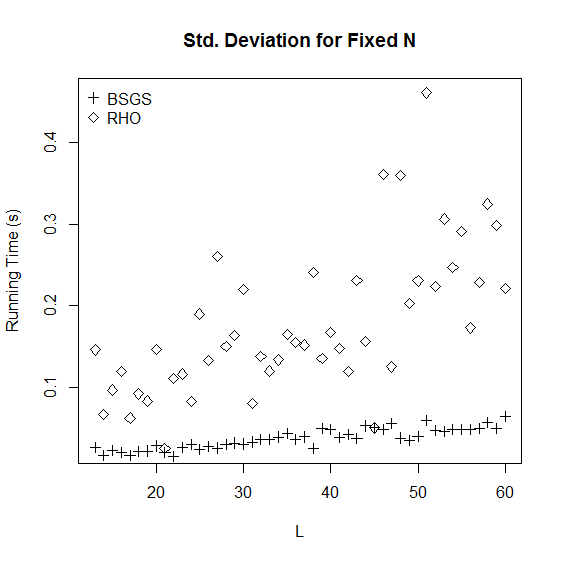
\includegraphics[angle=0, scale=0.55]{bab5/img/sdev-fixed-n}
	\caption{Grafik Standar Deviasi Kinerja Dua Metode Untuk Kelompok Masukan N Tetap}
	\label{fig:stddev_fixed_n}
\end{figure}

Pada grafik \ref{fig:stddev_fixed_n}, standar deviasi metode \textit{Pollard Rho} selalu berada di atas metode \textit{Baby-step Giant-step}. Standar deviasi metode \textit{Pollard Rho} juga relatif tinggi untuk kelompok masukan N tetap, namun masih di bawah batas atas permasalahan yaitu 1 detik. Di sisi lain, metode \textit{Baby-step Giant-step} memiliki standar deviasi yang kecil (kurang dari 0.1 detik). Artinya, metode \textit{Baby-step Giant-step} apabila digunakan untuk kelompok masukan N tetap akan menghasilkan \textit{running time} yang tidak jauh dari rata-rata \textit{running time} kelompok masukan N tersebut.

Secara umum, dampak besarnya L terhadap pertumbuhan \textit{running time} permasalahan untuk dua metode tersebut tidak begitu besar: hingga L terbesar yang mematuhi batasan soal, rata-rata \textit{running time} kedua metode tidak ada yang mencapai 1 detik. Selain itu, pertumbuhan fungsi rata-rata kedua metode cenderung linear.

\subsection{Pengujian Menggunakan Parameter Masukan dengan L Tetap}

Grafik perbandingan kinerja dua metode (\ref{fig:mean_fixed_l} dan \ref{fig:stddev_fixed_l})untuk parameter masukan dengan nilai $ L $ tetap.

\begin{figure}[h!]
	\Centering
	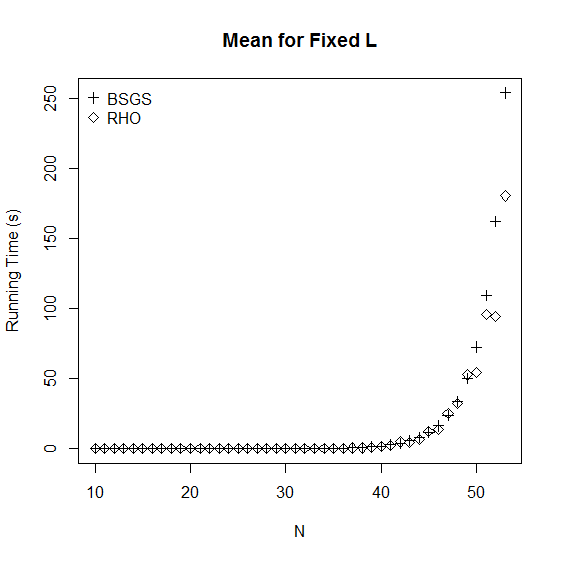
\includegraphics[angle=0, scale=0.55]{bab5/img/mean-fixed-l}
	\caption{Grafik Rata-rata Kinerja Dua Metode Untuk Kelompok Masukan L Tetap}
	\label{fig:mean_fixed_l}
\end{figure}

Grafik \ref{fig:mean_fixed_l} menunjukkan bahwa kedua metode memiliki pertumbuhan fungsi yang relatif sama. Pada $ N \geq 40 $, kedua grafik mulai melonjak naik. Namun terdapat sedikit perbedaan antar keduanya, yaitu metode rata-rata \textit{running time} \textit{Pollard Rho} lebih kecil daripada \textit{Baby-step Giant-step}. Berikutnya, grafik \ref{fig:stddev_fixed_l} akan menjelaskan mengenai standar deviasi kedua metode.

\begin{figure}[h!]
	\Centering
	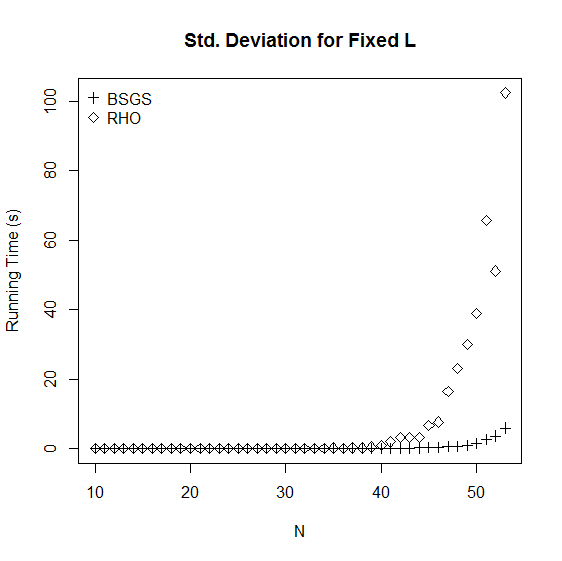
\includegraphics[angle=0, scale=0.55]{bab5/img/sdev-fixed-l}
	\caption{Grafik Standar Deviasi Kinerja Dua Metode Untuk Kelompok Masukan L Tetap}
	\label{fig:stddev_fixed_l}
\end{figure}

Berdasarkan grafik \ref{fig:stddev_fixed_l}, pertumbuhan fungsi standar deviasi kedua metode kontras dengan pertumbuhan fungsi rata-rata kedua metode. Pertumbuhan standar deviasi metode \textit{Pollard Rho} lebih besar dibanding metode \textit{Baby-step Giant-step}. Hal ini dapat dilihat pada $ N \geq 40 $.

Dari kedua pengujian kinerja terdapat kesamaan antara kedua metode terlepas dari jenis masukan yang digunakan.

\begin{enumerate}
	\item Rata-rata kinerja metode \textit{Baby-step Giant-step} dan \textit{Pollard Rho} relatif sama
	\item Standar deviasi metode \textit{Pollard Rho} cenderung lebih tinggi daripada \textit{Baby-step Giant-step}
	\item Fungsi pertumbuhan standar deviasi suatu metode sama dengan fungsi pertumbuhan rata-rata metode tersebut
\end{enumerate}

Selain itu berdasarkan uji kinerja dapat ditarik beberapa kesimpulan terkait waktu yang dibutuhkan untuk menyelesaikan permasalahan.

\begin{enumerate}
	\item Penyelesaian permasalahan dengan \textit{Baby-step Giant-step} akan membutuhkan waktu yang mendekati rata-rata \textit{running time} untuk kelompok masukan tersebut
	\item Penyelesaian permasalahan dengan \textit{Pollard Rho} dapat berjalan jauh lebih cepat atau jauh lebih lambat dari rata-rata \textit{running time} untuk kelompok masukan tersebut
	\item Besarnya L memiliki pengaruh yang tidak begitu signifikan terhadap lamanya waktu penyelesaian
	\item Besarnya N memiliki pengaruh yang signifikan terhadap lama waktu penyelesaian
\end{enumerate}